\documentclass[12pt]{article}
\usepackage[utf8]{inputenc}

\usepackage{lmodern}

\usepackage{enumitem}
\usepackage[margin=2cm]{geometry}

\usepackage{amsmath, amsfonts, amssymb}
\usepackage{graphicx}
%\usepackage{subfigure}
\usepackage{tikz}
\usepackage{pgfplots}
\usepackage{multicol}

\usepackage{comment}
\usepackage{url}
\usepackage{calc}
\usepackage{subcaption}
\usepackage[indent=0pt]{parskip}
\usepackage{animate}

\usepackage{array}
\usepackage{blkarray,booktabs, bigstrut}
\usepackage{bigints}

\pgfplotsset{compat=1.16}

% MATH commands
\newcommand{\ga}{\left\langle}
\newcommand{\da}{\right\rangle}
\newcommand{\oa}{\left\lbrace}
\newcommand{\fa}{\right\rbrace}
\newcommand{\oc}{\left[}
\newcommand{\fc}{\right]}
\newcommand{\op}{\left(}
\newcommand{\fp}{\right)}

\newcommand{\bi}{\mathbf{i}}
\newcommand{\bj}{\mathbf{j}}
\newcommand{\bk}{\mathbf{k}}
\newcommand{\bF}{\mathbf{F}}

\newcommand{\mR}{\mathbb{R}}

\newcommand{\ra}{\rightarrow}
\newcommand{\Ra}{\Rightarrow}

\newcommand{\sech}{\mathrm{sech}\,}
\newcommand{\csch}{\mathrm{csch}\,}
\newcommand{\curl}{\mathrm{curl}\,}
\newcommand{\dive}{\mathrm{div}\,}

\newcommand{\ve}{\varepsilon}
\newcommand{\spc}{\vspace*{0.5cm}}

\DeclareMathOperator{\Ran}{Ran}
\DeclareMathOperator{\Dom}{Dom}

\newcommand{\exo}[1]{\noindent\textcolor{red}{\fbox{\textbf{Problem {#1}}}\hrulefill}\\}
\newcommand{\qu}[4]{\noindent\textcolor{#4}{\fbox{\textbf{Section {#1} | Problem {#2}}} \hrulefill{{\fbox{\textbf{{#3} Points}}}}\\}}

\newcommand{\semester}{Spring 2023}

\newcommand{\CVup}{%
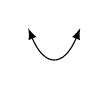
\begin{tikzpicture}
\draw[black, <->, >=latex] (-0.33, 0.5) .. controls (-0.125, 0) and (0.125, 0) .. (0.33, 0.5);
\end{tikzpicture}}

\newcommand{\CVupInc}{%
\begin{tikzpicture}
\draw[black, ->, >=latex] (0,0) .. controls (0.2, 0) and (0.4, 0.2) .. (0.5, 0.5);
\end{tikzpicture}}

\newcommand{\CVupDec}{%
\begin{tikzpicture}[rotate=270]
\draw[black, ->, >=latex] (0,0) .. controls (0.2, 0) and (0.4, 0.2) .. (0.5, 0.5);
\end{tikzpicture}}

\newcommand{\CVdown}{%
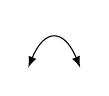
\begin{tikzpicture}
\draw[black, <->, >=latex] (-0.33, -0.5) .. controls (-0.125, 0) and (0.125, 0) .. (0.33, -0.5);
\end{tikzpicture}}

\newcommand{\CVdownInc}{%
\begin{tikzpicture}
\draw[black, ->, >=latex] (-0.5, -0.5) .. controls (-0.5, -0.3) and (-0.5, -0.1) .. (0,0);
\end{tikzpicture}}

\newcommand{\CVdownDec}{%
\begin{tikzpicture}[rotate=-90]
\draw[black, ->, >=latex] (-0.5, -0.5) .. controls (-0.5, -0.3) and (-0.5, -0.1) .. (0,0);
\end{tikzpicture}}

\begin{document}
	\noindent \hrulefill \\
	MATH-241 \hfill Pierre-Olivier Paris{\'e}\\
	Solutions Section 5-3 \hfill \semester \\\vspace*{-1cm}
	
	\noindent\hrulefill
	
	\spc
	
	\exo{16}
	\\
	Here is the sketch of the region to rotate about the axis $x = 3$:
		\begin{figure}[h]
		\begin{subfigure}[b]{0.45\textwidth}
		\centering
		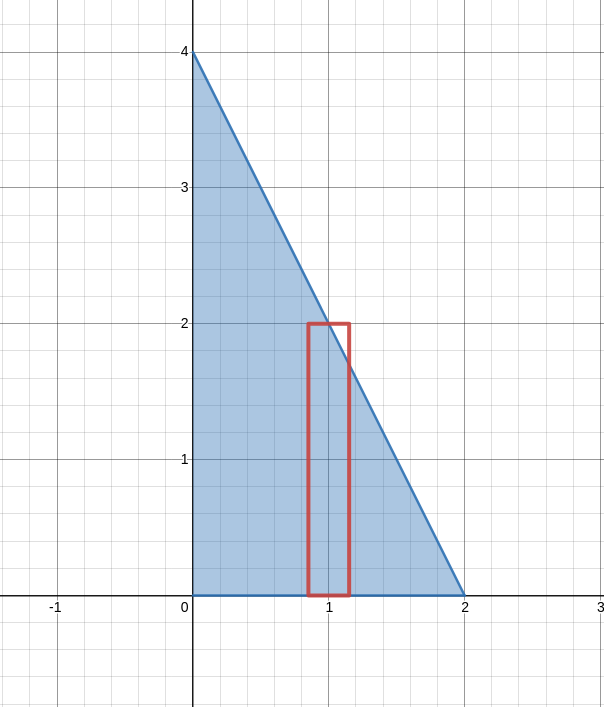
\includegraphics[scale=0.3]{5-3_exo16}
		\caption{Region to rotate}
		\end{subfigure}
		\begin{subfigure}[b]{0.45\textwidth}
		\animategraphics[scale=0.75]{20}{python_5-3_16/Revolution}{0}{200}
		\caption{Rotation of the region}
		\end{subfigure}
		\end{figure}
	
	We will use the cylindrical shells method. The radius is $x + 1$ and the height is $y$ and the limits are $0 \leq x \leq 2$. Thus, we get
		\begin{align*}
		V(S) = \int_0^2 2\pi (x + 1) y \, dx = 2\pi \int_0^2 (x + 1) (4 - 2x) \, dx = 20/3 .
		\end{align*}
	
	\newpage
	
	\exo{18}
	\\
	The region is bounded by the curves
		\begin{align*}
		y = \sqrt{x} \quad \text{ and } \quad x = 2y .
		\end{align*}
	Therefore, the curve meets when
		\begin{align*}
		\sqrt{x} = \frac{x}{2} \iff x = \frac{x^2}{4} \iff \frac{1}{4} x (x- 4) = 0 \iff x = 0 \text{ or } x = 4 .
		\end{align*}
	A sketch of the region is presented below with a typical rectangle to generate the spherical shell:
	\begin{center}
	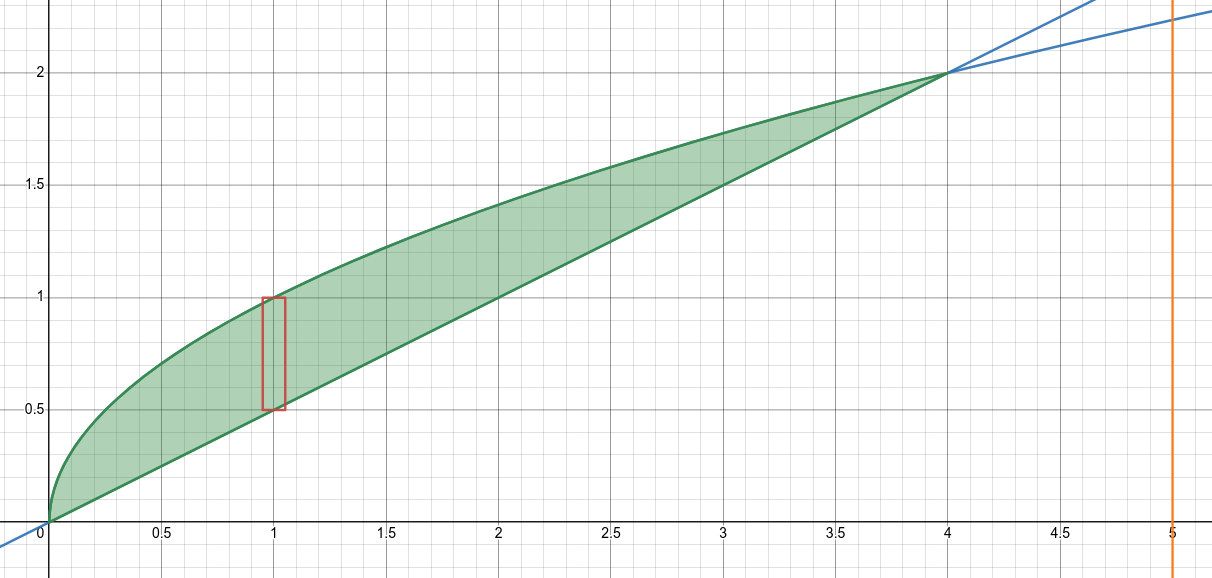
\includegraphics[scale=0.4]{fig5.png}
	\end{center}
	
	After rotating about the line $x = 5$, we obtain a cylindrical shell with
		\begin{itemize}
		\item height: $\sqrt{x} - \frac{x}{2}$;
		\item radius: $5 - x$;
		\item thickness: $dx$.
		\end{itemize}
	Therefore, the volume is given by
		\begin{align*}
		\int_a^b 2\pi (\text{radius}) (\text{height}) \, dx = \int_0^4 2\pi (5-x) \big(\sqrt{x} - \frac{x}{2} \big) \, dx
		\end{align*}
	The value of this integral is the volume of the solid of revolution. Therefore, the volume of the solid of revolution is $\frac{136}{15} \pi$.
	
	\newpage
	
	\exo{30}
	\\
	The radius is $y$ and the height is $x = \sqrt{y - 1}$ and the limits are $1 \leq y \leq 5$. So, the solid is obtained by rotating the following region around the $x$ axis:
		\begin{figure}[h]
		\centering
		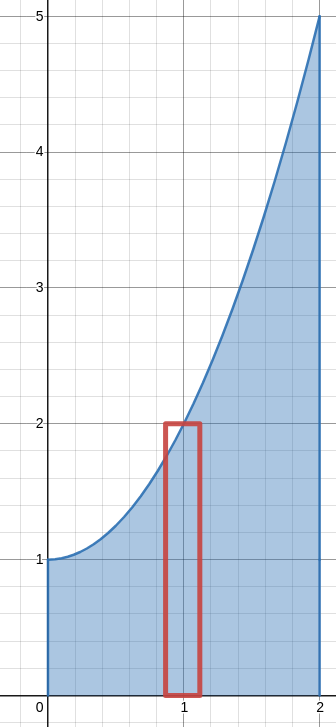
\includegraphics[scale=0.3]{5-3_exo30}
		\end{figure}
	
\end{document}